\chapter{Methodology}
\label{methodology}

In this chapter,
the methodological approach,
as well as
the used scientific research methods
are presented.





\section{Motivation and Objectives}
\label{methodology:motivation-and-objectives}

%TODO: motivation and goal of this chapter ; introduction to what happens in this chapter

The chapter \nameref{methodology} starts off with an outline and brief description
of each activity of the general approach of this concrete research.
The research approach is framed around the design science research methodology by
\autocite{designScienceResearchMethodologyForInformationSystemsResearch},
which builds a structure and guideline in which the whole research is based on.
The purpose of following this methodological framework is to help with the recognition and
legitimization of the conducted research.
For certain activities, the semi-structured interview is used as a scientific method,
and for the core of the research, namely the development of a software artifact,
the prototyping method is applied.

All the used research methods are described,
and especially how exactly they are applied within this thesis.

Finally the chapter ends with a summary of what has been presented,
as well as the key takeaways, which are needed for comprehension of the following chapters of this thesis.





\section{General Approach}
\label{methodology:approach}

To achieve the main goal of the thesis and answer the identified research questions,
a mix of different scientific methods will be used.
In order to help with the recognition and legitimization of the conducted research,
a commonly accepted framework, namely
the methodology for conducting design science (DS) research
in information systems (IS)
\autocite{designScienceResearchMethodologyForInformationSystemsResearch}
will be applied.
It consists of six activities
(illustrated in Figure \ref{fig:dsrmProcessReleasePromotionGitOps}):

\begin{itemize}
	\item \nameref{methodology:activity1}
	\item \nameref{methodology:activity2}
	\item \nameref{methodology:activity3}
	\item \nameref{methodology:activity4}
	\item \nameref{methodology:activity5}
	\item \nameref{methodology:activity6}
\end{itemize}

%Since the model allows for process iteration,
%it will be decided by the researcher
%whether, at the end of activity 5,
%to iterate back to activity 3 to try to improve the artifact.
The process is structured in a nominally sequential order.
For this concrete research,
the problem-centered initiation is chosen as the entry point,
thus the process will begin with activity 1.
Afterwards the research will proceed sequentially,
because the idea of the research resulted from observation of the problem
\autocite{designScienceResearchMethodologyForInformationSystemsResearch}.
\bigskip

% TODO: add activity 1-6 to illustration?

\begin{figure}[h]
	\centering
	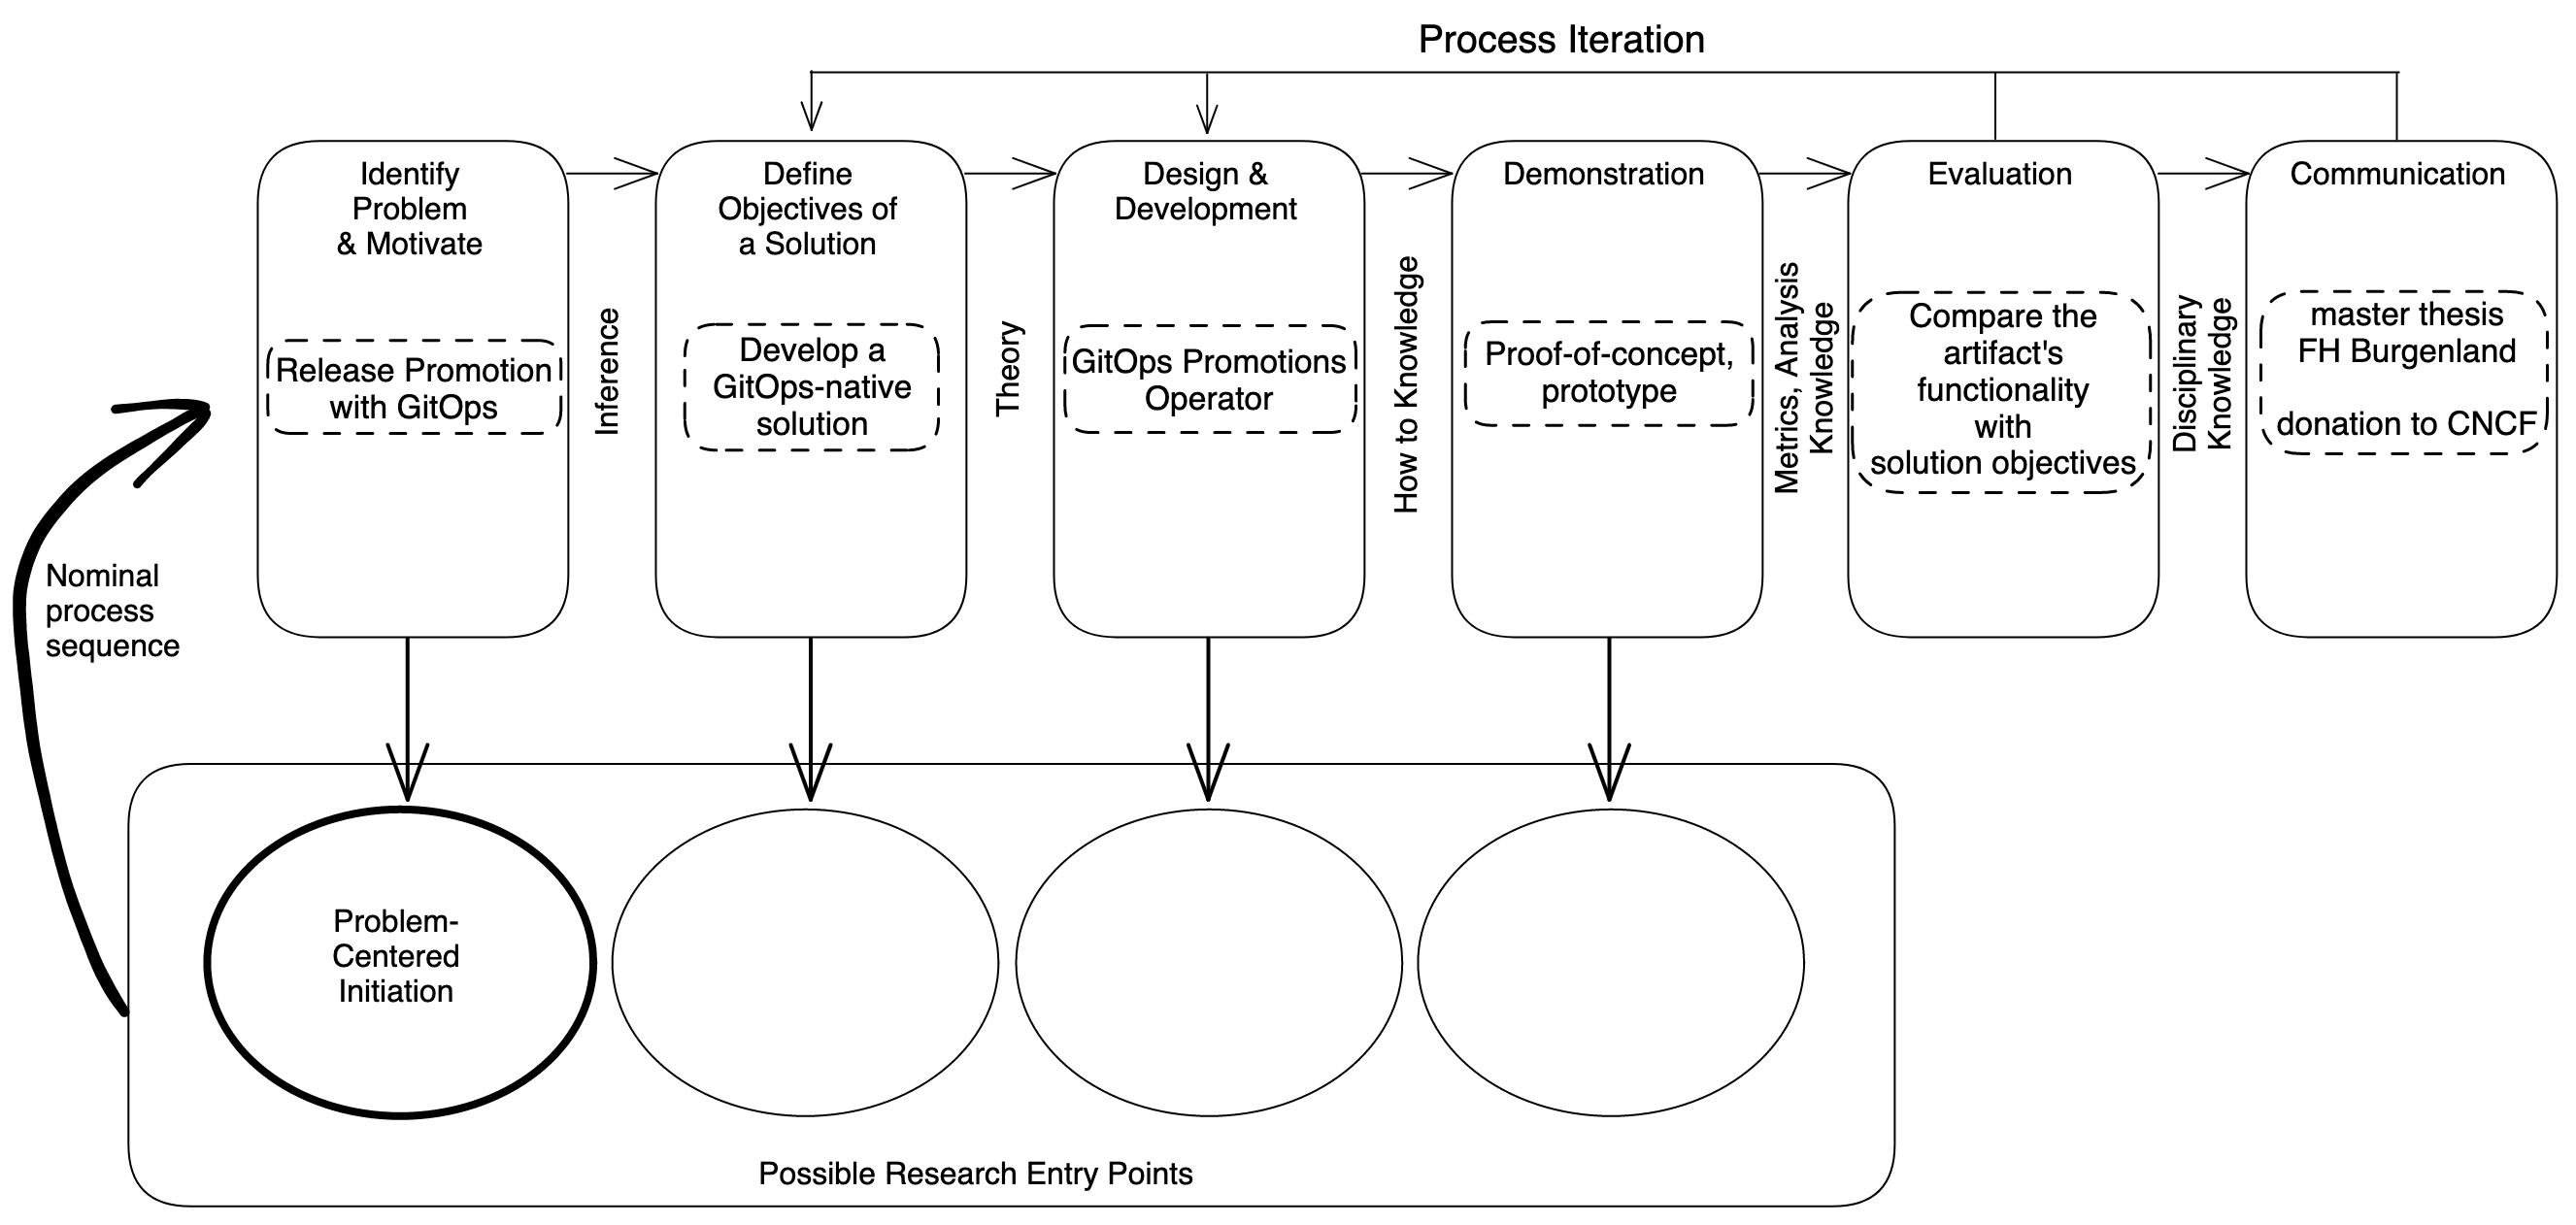
\includegraphics[width=1.00\linewidth]{figures/dsrm-process-release-promotion-gitops.png}
	\caption{DSRM Process for this thesis.
		%		(\citeauthor{ref}, \citeyear{ref}).
	}
	\label{fig:dsrmProcessReleasePromotionGitOps}	
\end{figure}

\subsection{Activity 1: Identify Problem \& Motivate}
\label{methodology:activity1}

\noindent
In activity 1,
the research problem of
release promotion with GitOps
is defined.
This is accomplished, by
seeking knowledge of the state of the problem
from practicing professionals.
This is done by conducting
semi-structured interviews, as described in section \ref{methodology:interview},
as well as analysing prior written literature.
To assist later evaluation,
the problem is conceptually broken down into distinct items.
The value of a solution is highlighted,
in order to help the audience of the research
understand the reasoning associated with the
researcher's understanding of the problem
\autocite{designScienceResearchMethodologyForInformationSystemsResearch}.
\bigskip

\begin{figure}[h]
	\centering
	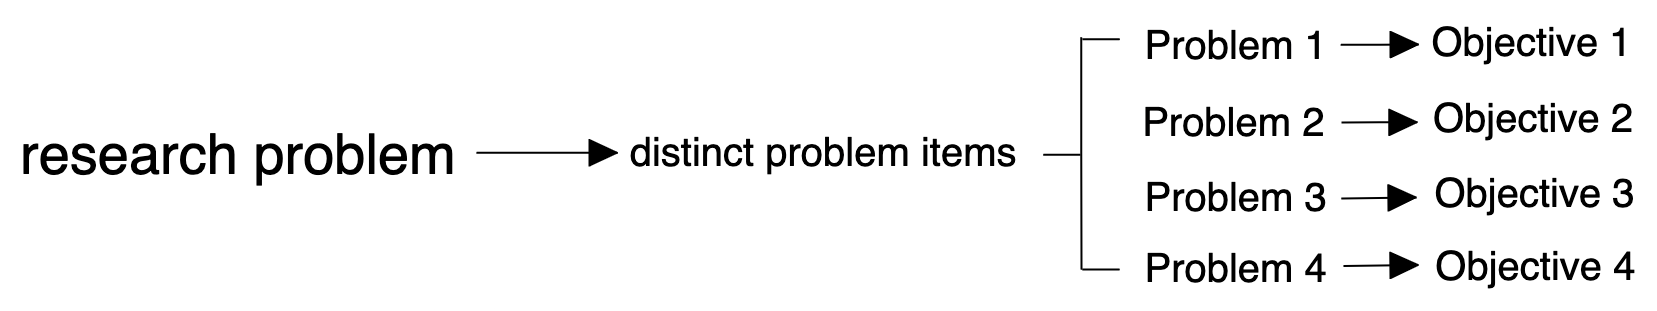
\includegraphics[width=0.75\linewidth]{assets/problem-to-objective-mapping.png}
	\caption{Inference of objectives from problems.
		%		(\citeauthor{ref}, \citeyear{ref}).
	}
	\label{fig:problemToObjectiveMapping}	
\end{figure}

\subsection{Activity 2: Define Objectives of a Solution}
\label{methodology:activity2}

\noindent
In activity 2,
research objectives are inferred from the problem definition in activity 1.
Each objective maps to a distinct item from the problem specification
(illustrated in Figure \ref{fig:problemToObjectiveMapping}),
which helps with later evaluation in activity 5.
In practice, a research objective will be a qualitative description of
how a new artifact is expected to support a solution to the problem definition.
\bigskip

\subsection{Activity 3: Design \& Development}
\label{methodology:activity3}

\noindent
In activity 3,
solutions for the previously defined objectives are designed and developed
by means of producing an artifact.
This is achieved by
determining the artifact's desired functionality and its architecture,
followed by actually creating the artifact
\autocite{designScienceResearchMethodologyForInformationSystemsResearch}.
In practice this means that:
Abstract model definitions are designed;
with the specification of the model definitions in place,
the GitOps Promotions Operator prototype is developed as an artifact.
\bigskip

\subsection{Activity 4: Demonstration}
\label{methodology:activity4}

\noindent
In activity 4,
the in-context use of the artifact is demonstrated in a proof of concept.
%After outlining how to use the artifact to effectively provide a solution to the problem definition,
%the artifact is implemented in a proof-of-concept-level prototype.
%
%In practice,
%the prototype 
\bigskip

\subsection{Activity 5: Evaluation}
\label{methodology:activity5}

\noindent
In activity 5,
the implementation of the artifact,
and how well it supports a solution to the problem,
is evaluated.
This is achieved by
comparing the objectives of a solution to actual observed results
from use of the artifact in the demonstration
\autocite{designScienceResearchMethodologyForInformationSystemsResearch}.
In practice this means, that
the functionality of the artifact implemented in the prototype in activity 4,
is compared with the solution objectives from activity 2.
\bigskip

\subsection{Activity 6: Communication}
\label{methodology:activity6}

\noindent
In activity 6, as a final step,
the whole conducted research is communicated by means of
disclosing
the problem and its importance,
the artifact and its utility and novelty,
and the demonstration accompanied by the evalution results
\autocite{designScienceResearchMethodologyForInformationSystemsResearch},
within the publication of a master thesis at
the University of Applied Sciences Burgenland \autocite{fhBurgenlandWebsite}.
In addition, it is communicated to relevant audiences such as
the GitOps Working Group \autocite{gitopsWG} of the CNCF.






\section{Research methods}

In the following section,
the used research methods
semi-structured interview
%and qualitative content analysis
by
\citeauthor{glaser2010experteninterviews} (\citeyear{glaser2010experteninterviews}),
design science research methodology for information systems
by
\citeauthor{designScienceResearchMethodologyForInformationSystemsResearch} (\citeyear{designScienceResearchMethodologyForInformationSystemsResearch}),
and prototyping as described
by
\citeauthor{riedlManagementInformatik2019} (\citeyear{riedlManagementInformatik2019})
are explained in detail.

%The procedure in the course of the research work is also described.




\subsection{Semi-structured Interview}\label{methodology:interview}

For \nameref{methodology:activity1},
semi-structured interviews with working professionals
are conducted.
For this research method,
the suggested practices and guidelines from
the textbook of
\citeauthor{glaser2010experteninterviews} (\citeyear{glaser2010experteninterviews})
are used.
These interviews have the primary goal of aiding with
problem identification and motivation,
because prior written scientific literature is insufficient on the topic.
For conducting the interviews,
a semi-structured interview guide (Appendix \ref{appendix:interview-guide}) is used.

The interview guide is created on the basis of preliminary theoretical considerations.
The use of a guide facilitates the comparability of several interviews,
but still leaves enough room for spontaneous statements.
The advantage of a guide is that the researcher can stick to concrete questions.
Follow-up questioning is allowed and the questions are mostly open.
The open questioning enables the interviewee to present their point of view
\autocite{berger2016wissenschaftliches}.


\subsubsection*{Preparing the Interviews}

As an initial step,
a semi-structured interview guide is developed.
It serves as a rough guideline for the structure of the interview process.
Additionally it encompasses the content-related interview questions,
which are specific to the given research problem.
These questions can be seen at section \ref{appendix:interview-questions} in the appendix.

The selection of the interview partners is based on the questions mentioned in
\citeauthor{glaser2010experteninterviews} (\citeyear{glaser2010experteninterviews}):

\begin{itemize}
	\item Who has the information relevant to this work?
	\item Who can describe it precisely?
	\item Who is most willing to be interviewed?
	\item Who is available?
\end{itemize}

The pool of potential interview partners is mainly oriented around
contacts from friends and acquaintances,
who are working professionally in the GitOps field.
The contact to the interview partners is done via Slack \autocite{slackWebsite} or e-mail.
Prior to conducting the interview, the interview guide is sent to the interviewee.

\subsubsection*{Conducting the interviews}

Appointments for the interviews are made with each interview partner in advance. 
Eventually, the interview is conducted with a web video conferencing tool like Zoom \autocite{zoomWebsite}.
The interviews are recorded for later transcription.
The semi-structured interview guide
is used as a guideline for the interview process as a whole.
However, the actual structure of the interview may differ for each individual interview and according interview partner.

\subsubsection*{Transcription and post-processing of the interviews}

The output of the interviews are in the form of audio-video recordings.
These are transcribed word-for-word into a written form afterwards.
The transcriptions can be seen in Appendix \ref{appendix:interview-transcriptions}.
The content-related answers of the interview partners are taken into consideration
for \nameref{methodology:activity1}, and there further processed.




%
%\subsection{Qualitative Content Analysis}
%
%For \nameref{methodology:activity2},
%the transcriptions of the interviews are evaluated with
%the qualitative content analysis by
%\citeauthor{mayring2019qualitative} (\citeyear{mayring2019qualitative}).
%
%\subsubsection*{Object and research question}
%
%The underlying object for the content analysis are
%the conducted semi-structured interviews as described in section \ref{methodology:interview}.
%
%The research questions are presented in the earlier section \ref{introduction:research-question}.
%
%\subsubsection*{Approach}
%
%As the main approach,
%the inductive category formation
%is chosen.
%The first text passage is read,
%then a category is formed,
%and finally the next passage is processed.
%For the next passage,
%it is to be decided if an existing category matches
%or a new one needs to be formed.
%This process continues until all text passages are handled.
%At the end, similar categories may be merged together.
%
%\subsubsection*{Coding}
%
%Each text passage is labelled with the according category.
%
%\subsubsection*{Review of categories}
%
%About halfway through the coding process,
%\citeauthor{mayring2019qualitative} (\citeyear{mayring2019qualitative})
%advises to review the already formed categories.
%The following questions may be asked:
%Do they represent the content well?
%Were they formed in an appropriate relation?
%How do possible denotations look?
%Could you merge certain categories
%\autocite{mayring2019qualitative}?
%
%\subsubsection*{Completion of coding process}
%
%After reviewing the categories,
%and taking appropriate measures,
%the coding process is completed.
%
%\subsubsection*{Reliability check}
%
%Once coding is completed,
%a reliability check is done.
%How much do the results differ in replication?
%This is achieved by letting another independent researcher
%execute the coding process.
%
%%Cohens's Kappa (1960)
%%Krippendorff's Alpha (1970)
%
%\subsubsection*{Evaluation and interpretation}
%
%A possible way for evaluation would be to check frequencies.
%
%How often does each of the categories occur in the data set?
%What does this mean in terms of the research question?
%How do the results relate to the existing state of research?













\subsection{Design Science Research Methodology}

The
design science research methodology (DSRM)
has already been thoroughly described and applied in the earlier section
\ref{methodology:approach} \nameref{methodology:approach}
of this thesis.
A concise definition is stated here nontheless.

\citeauthor{designScienceResearchMethodologyForInformationSystemsResearch} (\citeyear{designScienceResearchMethodologyForInformationSystemsResearch})
describe DSRM as follows:

\begin{quotation}
\noindent
\enquote*{We propose and develop a design science research methodology (DSRM) for the
production and presentation of DS research in IS. This effort contributes to IS research
by providing a commonly accepted framework for successfully carrying out DS research
and a mental model for its presentation. It may also help with the recognition
and legitimization of DS research and its objectives, processes, and outputs, and it
should help researchers to present research with reference to a commonly understood
framework, rather than justifying the research paradigm on an ad hoc basis with each
new paper.}
\autocite{designScienceResearchMethodologyForInformationSystemsResearch}
\end{quotation}

\enquote*{DS is of importance in a discipline oriented to the creation of successful artifacts.}
\autocite{designScienceResearchMethodologyForInformationSystemsResearch}


%DSRM provides a nominal process model consisting of six steps:
%problem identification and motivation, definition of the objectives for a solution, design and development, demonstration, evaluation, and communication






\subsection{Prototyping}
\label{methodology:prototyping}

For the research method prototyping,
which is applied in
\nameref{methodology:activity3}
and
\nameref{methodology:activity4},
the literature of \citeauthor{riedlManagementInformatik2019} (\citeyear{riedlManagementInformatik2019}) is used.

The terms prototype, prototyping, prototyping cycle and phase scheme are defined in the earlier chapter
\ref{theoretical-background:general-definitions} \nameref{theoretical-background:general-definitions}
of this thesis.

\subsubsection*{Types of Prototypes}

There are several different types of prototypes,
however they each share common traits.
A prototype
\autocite{riedlManagementInformatik2019}

\begin{itemize}
	\item can be developed quickly and at a low-cost.
	\item provides a functional and executable model for evaluation by future users before actual implementation.
	\item is easy to modify and extend.
	\item does not necessarily represent the system completely.
	\item serves as a means of communication between the developers and the users.
	\item can be evaluated by all stakeholders involved in the planning process.
\end{itemize}

According to the type of prototype, a distinction is made between complete and incomplete prototypes
as well as disposable and reusable prototypes
\autocite{riedlManagementInformatik2019}.

A \textbf{full prototype} is a prototype that makes all the essential functions of the information system to be created fully available.
The experience gained during planning and during use and the prototype itself form the basis for the final system specification
\autocite{riedlManagementInformatik2019}.

An \textbf{incomplete prototype} is a prototype that allows the usability and/or feasibility of individual components
of the information system to be created (e.g., the user interface) to be assessed
\autocite{riedlManagementInformatik2019}.

A \textbf{disposable prototype} is a prototype that serves only as an executable model;
it is not used directly for the information system to be created
\autocite{riedlManagementInformatik2019}.

A \textbf{reusable prototype} is a prototype that meets all quality requirements and from which
essential parts can be adopted in the information system to be created
\autocite{riedlManagementInformatik2019}.

%

Another systematic approach, based primarily on the intended use of the prototype, distinguishes between demonstration prototype, laboratory sample and pilot system
\autocite{riedlManagementInformatik2019}.

The \textbf{demonstration prototype} supports project initiation or project acquisition; it should convince the potential client that the desired end product can be built or that its handling corresponds to what the future users imagine. A prototype for this purpose therefore has the characteristics of the incomplete prototype and usually also of the disposable prototype
\autocite{riedlManagementInformatik2019}.

The \textbf{laboratory sample} is primarily used to clarify design-related issues; it is derived from the model of the application task and from an existing specification. The design of the end product should be essentially identical, or at least comparable, to that of the laboratory prototype. This requirement can refer to the architecture and/or to the functionality.
\autocite{riedlManagementInformatik2019}.

In the \textbf{pilot system}, the strict separation between prototype and end product is eliminated. At a certain level of maturity, the prototype is used productively at individual workplaces and is further developed. It is initially incomplete and reusable; as it matures, it becomes complete
\autocite{riedlManagementInformatik2019}.

%

For the concrete research of this thesis,
The type \textbf{demonstration prototype} is used.

\subsubsection*{Evaluation of Prototypes}

Evaluating prototypes presupposes that there is an evaluation strategy agreed between the developers on the one hand
and the users on the other; prototypes must be developed with the evaluation strategy in mind.
The evaluation strategy specifies the what and the how of the evaluation.
This includes agreements on the time intervals in which modified versions of the prototype are made available for evaluation (evaluation cycle).
From a methodological point of view, short evaluation cycles are preferable in order to quickly stabilize the requirements.
This intensifies communication between the partners and promotes user participation.
The what of the evaluation makes statements about which properties the prototype should have
(especially with regard to functions, services and interfaces).
The what of the evaluation strategy indicates which properties the final product should have and which properties are specific to the prototype
(or to several versions of the prototype) and are therefore only preliminary.
The how of the evaluation makes statements about which evaluation method should be used to arrive at a result that is accepted by both partners.
In general, a procedure according to the model of utility analysis is appropriate, which is adapted to the object of evaluation
and coordinated with the evaluation situation. This requires agreements on how different results of the evaluation are to be treated
by the developers on the one hand and the users on the other hand. The goal is to achieve agreement
\autocite{riedlManagementInformatik2019}.

For the concrete research of this thesis,
several disposable prototypes are developed
by the researcher.
Some parts are reusable for next iterations.
Finally a reusable but incomplete prototype is evaluated against the research objectives,
together with the interview partners (potential users).
A thorough evaluation of the prototype with a high amount of users is not done,
due to the time and effort constraints of this thesis.

\subsubsection*{Types of Prototyping}

Types of prototyping means why prototypes are used and fundamentally how to proceed with their usage.
A distinction is then made between \textbf{exploratory}, \textbf{experimental} and \textbf{evolutionary prototyping}.

\textbf{Exploratory prototyping} aims to determine the functional requirements of an information system by developing a prototype that allows for testing of different solution alternatives with users.
The future users should be able to evaluate the prototype on the basis of real work situations.
The focus is on functionality, ease of change, and short development time.
The required functions are determined successively.
The influence on the phase scheme is minimal as it's primarily used for requirements analysis.

\textbf{Experimental prototyping} aims to complete the specification of system components and
prove the suitability of object specifications, architecture models, and solution ideas.
Users are not usually involved in this process, and implementation work is integrated ("pulled forward") into analysis and design work,
which changes the phase scheme more than exploratory prototyping.
Sometimes the use of prototypes for evaluation by users is described as "experimenting with prototypes";
this is concluded as experimental prototyping
\autocite{riedlManagementInformatik2019}.

Finally, \textbf{evolutionary prototyping} is an incremental project work approach that involves developing 
a prototype for easily identifiable requirements, which is then used as the basis for the next planning step. 
The prototype and information system become indistinguishable as the prototype is successively improved 
and ultimately used as a productive information system. 
The change in the phase scheme is most apparent in evolutionary prototyping
\autocite{riedlManagementInformatik2019}.

For the concrete research of this thesis,
a mix of all three prototyping types are applied,
as described in the following section.

\subsubsection*{Prototyping approach}

Prototyping results in an approach that modifies the phase scheme, but in no way substitutes it. Exploratory and experimental prototyping can be used "intermixed". A typical approach is the following: First, an explorative approach is taken, for which a disposable prototype is created (rapid prototyping, also referred to as quick and dirty). The primary goal is to minimize the time in which the first prototype is available. If the assessment shows that the essential requirements have been captured and taken into account, the prototype is only used for comparison purposes (e.g. to be able to check later whether the essential requirements have been updated). After that, an evolutionary approach is taken, for which a reusable prototype is developed. After each assessment, a decision is made as to what will better support the achievement of the planning goals: to modify the existing prototype or to discard it. If an evolutionary approach is taken and the prototype is reused in any case, then the following work steps can be distinguished
\autocite{riedlManagementInformatik2019}:

\begin{enumerate}
	\item rough specification of requirements
	\item creating a prototype
	\item using the prototype
	\item evaluating the prototype
	\item modify the prototype according to the results of the third step; run through the third and fourth steps n times
\end{enumerate}

After the prototype has been run through (n+1) times in the third to fifth steps (prototyping cycle), the final product has been created. A prototyping cycle can serve a specific purpose according to plan (e.g. a first cycle of initiation). Here, the primary purpose is for the participants to familiarize themselves with the project task. In the first prototype, therefore, only a few functions already known to the developers are realized. A second prototyping cycle can serve as orientation. The aim here is to capture all the essential requirements that will be realized in the prototype. Finally, a third purpose is stabilization. This is primarily about refining and adding features and producing the required performance. Late orientation and early stabilization prototypes are close to the level of the final product; they can therefore also be used for user training. If planning and realization of an information system are seen as a layer model, then prototyping can be done either horizontally or vertically. In horizontal prototyping, individual layers of the system are constructed (e.g., the user interface or the functions); in general, horizontal prototyping refers to the construction of the user interface. In vertical prototyping, a selected part of the target system is implemented "in depth". This approach is appropriate when the functionality of the overall system is unknown and its realization possibilities are questionable
\autocite{riedlManagementInformatik2019}.

For the concrete research of this thesis,
a mix of approaches is used.
First,
an experimental approach is taken
by developing several disposable software prototypes.
This is done in order to assess the essential technical requirements
and get a feel for the feasibility of the possible features (research objectives).
Then,
exploratory prototyping is used,
by evaluating the thus far developed prototype against the solution objectives
together with the interview partners (potential users).
Finally,
an evolutionary approach is taken,
for which a reusable prototype is developed.
Parts of the software prototype may be fully reused for future iterations.

\subsubsection*{Effects of prototyping}

\citeauthor{riedlManagementInformatik2019} (\citeyear{riedlManagementInformatik2019})
notes that on the effects of prototyping there is limited empirical evidence available.
Field reports suggest that the costs of prototyping can either increase or decrease,
depending on the context, type of costs, and type of prototype used.
However, some researchers argue that prototyping can reduce development costs
by providing early error detection and motivation for users, among other benefits.
The most significant effect of prototyping is seen in the improvement of the end product's functionality and usability,
resulting from improved cooperation between users and developers.
This can lead to better acceptance of the product by users, resulting in a decreased need for maintenance.
Additionally, the evaluation of prototypes can support project controlling and help assess whether
an IT project should be continued unchanged, rehabilitated with significant changes, or terminated altogether
\autocite{riedlManagementInformatik2019}.





\section{Summary}

TODO




















%\section{Approach}
%Alle im durchgeführten Untersuchungen und Versuche müssen systematisch und
%nachvollziehbar sein. Daher ist die gewählte Vorgangsweise genau zu beschreiben
%und zu begründen. Es empfiehlt sich, dafür Literatur zum wissenschaftlichen Arbeiten
%heranzuziehen.
%
%\section{Research methods}
%Die eingesetzte Methoden (z.B. Online-Befragung, Inhaltsanalyse, Interviews) müssen
%ebenfalls nachvollziehbar beschrieben werden.
%Unterschiedliche Untersuchungsmethoden haben oft unterschiedliche Genauigkeit.
%Neben der Begründung und Beschreibung der Untersuchungsmethoden ist auch eine
%Begründung und Beschreibung der verwendeten Auswertungsmethoden bzw. dafür
%verwendete Software unerlässlich\footnote{Wenn der Abstand zwischen Fußnotentrennstrich und Fußnote zu groß wird, gehen Sie folgend vor:
%	Wählen Sie im Hauptmenü „Ansicht | Entwurf | Verweise | Notizen anzeigen |
%	Fußnotentrennlinie". Dann können Sie unnötige Leerzeichen entfernen.
%}.
%Wenn es ein Kapitel 3.2.1 gibt, muss es auch ein Kapitel 3.2.2 geben.

%\subsubsection{<<Überschrift 4. Ebene>>}
%4 Überschriftenebenen müssen reichen.
%
%
%\section{Displayed Text}
%Text is displayed by indenting it from the left
%margin.  Quotations are commonly displayed.  There
%are short quotations
%\begin{quote}
%	This is a short quotation.  It consists of a 
%	single paragraph of text.  See how it is formatted.
%\end{quote}
%and longer ones.
%\begin{quotation}
%	This is a longer quotation.  It consists of two
%	paragraphs of text, neither of which are
%	particularly interesting.
%	
%	This is the second paragraph of the quotation.  It
%	is just as dull as the first paragraph.
%\end{quotation}
%Another frequently-displayed structure is a list.
%The following is an example of an \emph{itemized}
%list.
%\begin{itemize}
%	\item This is the first item of an itemized list.
%	Each item in the list is marked with a ``tick''.
%	You don't have to worry about what kind of tick
%	mark is used.
%	
%	\item This is the second item of the list.  It
%	contains another list nested inside it.  The inner
%	list is an \emph{enumerated} list.
%	\begin{enumerate}
%		\item This is the first item of an enumerated 
%		list that is nested within the itemized list.
%		
%		\item This is the second item of the inner list.  
%		\LaTeX\ allows you to nest lists deeper than 
%		you really should.
%	\end{enumerate}
%	This is the rest of the second item of the outer
%	list.  It is no more interesting than any other
%	part of the item.
%	\item This is the third item of the list.
%\end{itemize}
%You can even display poetry.
%\begin{verse}
%	There is an environment 
%	for verse \\             % The \\ command separates lines
%	Whose features some poets % within a stanza.
%	will curse.   
%	
%	% One or more blank lines separate stanzas.
%	
%	For instead of making\\
%	Them do \emph{all} line breaking, \\
%	It allows them to put too many words on a line when they'd rather be 
%	forced to be terse.
%\end{verse}
%
%Mathematical formulas may also be displayed.  A
%displayed formula 
%is 
%one-line long; multiline
%formulas require special formatting instructions.
%\[  \Gamma \times  \psi = x'' + y^{2} + z_{i}^{n}\]
%Don't start a paragraph with a displayed equation,
%nor make one a paragraph by itself.
